\section{Introduction partielle}
Ce chapitre vient clore notre travail. Nous envisageons y présenter sommairement les éléments qu'il serait normalement nécessaire de concevoir pour réaliser un système de traitement numérique complet du signal. Toutefois, étant donné que notre travail consiste juste à élaboré le filtre, nous nous limiterons, pour les autres blocs de traitement du signal, à la description du minimum nécessaire pour comprendre l'ensemble. Ça veut dire que nous ne concevrons pas les autres parties, sinon nous nous serons totalement écarté du cadre de ce travail. Nous allons considérer que le reste est un acquis à ajuster seulement à la partie concernant le traitement que nous allons élaborer et implémenter sous \textbf{Matlab}.
\section{Structure globale du système}
Notre système fonctionne selon la procédure classique de traitement du signal. De ce fait, il sera constitué des blocs habituels. C'est ainsi que la structure globale du système est telle que représenté sur la figure qui suit:\newpage
\begin{center}
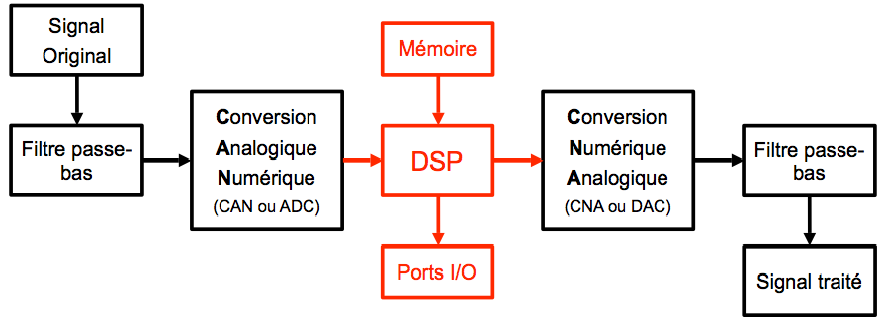
\includegraphics[scale=0.5]{EssaiImage.png}
\captionof{figure}{Chaîne typique de traitements du signal \cite{ImageChaineTrait}}
\end{center}
On y remarque que minimalement, un système de traitement complet devra contenir des éléments qui réalisent ces $ 5 $ étapes. A l'arrivée du signal il sera d'abord adapté au système, d'où le filtre anti-repliement. Ensuite, comme le traitement est numérique, il sera converti sous forme binaire par le Convertisseur Analogique-Numérique. Par après il subira un traitement adéquat (le filtrage numérique pour notre cas), puis la reconversion sous forme analogique grâce au convertisseur Numérique-Analogique. Finalement, on terminera la mise en forme du signal en le lissant grâce au filtre de lissage.
\subsection{Filtre anti-repliement}
\paragraph{}
Le filtre anti-repliement est nécessaire pour faire respecter le théorème de Shannon; il évite le repliement de spectre auquel on assiste normalement si la condition de Nyquist-Shannon est violée par sous-échantillonnage (c'est-à-dire si la fréquence d'échantillonnage est inférieure au double de la fréquence maximale du signal échantillonné). Ce phénomène est pourtant de règle et n'est en rien une exception vu que normalement, les signaux réels ne sont jamais, stricto sensu, à support fréquentiel borné. Donc, les spectres réels s'étendent toujours jusqu'à l'infini (l'amplitude du signal tendant bien sûr vers $ 0 $ sans jamais s'annuler). Par conséquent, la condition de Nyquist-Shannon ne peut jamais être strictement respectée pour un signal réel. D'où l'importance d'un filtre anti-repliement.\\
Le filtre n'est en effet qu'un passe-bas permettant de limiter la fréquence maximale prise par le signal à traiter pour que nous soyons sûr de choisir une fréquence d'échantillonnage valable (valeur non infinie).\\
Les figures \ref{NonRepliement} et \ref{OuiRepliement} nous présentent de façon imagées le répliement et l'absence de repliement.\newpage
\begin{center}
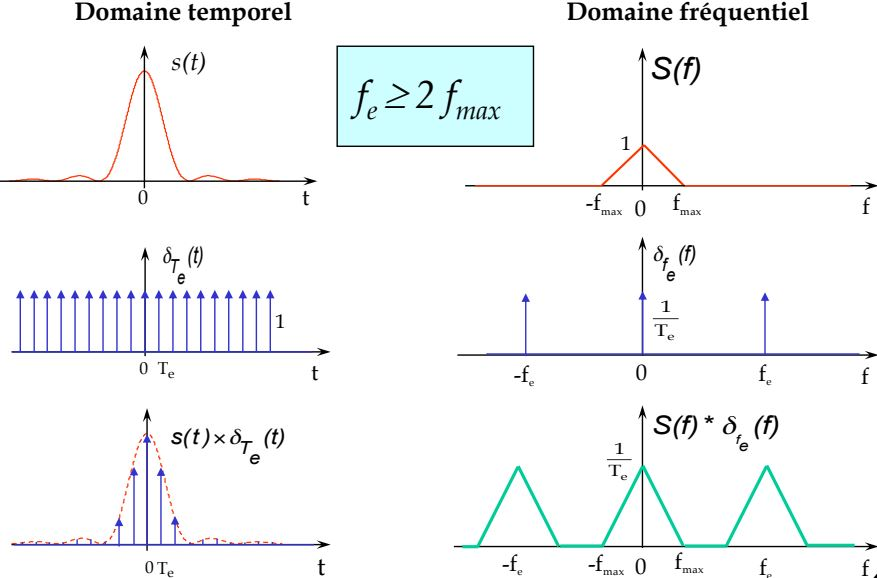
\includegraphics[scale=0.5]{nonReplie.jpg}
\captionof{figure}{Absence de repliement\cite{Tds}}\label{NonRepliement}
\end{center}
\begin{center}
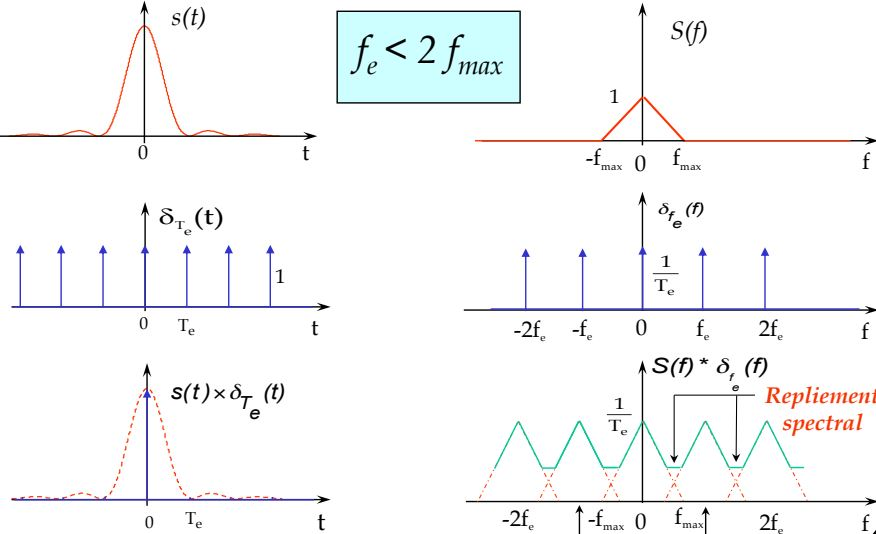
\includegraphics[scale=0.5]{Replie.jpg}
\captionof{figure}{Présence de repliement\cite{Tds}}\label{OuiRepliement}
\end{center}
\paragraph{}
Il est donc indispensable d'intercaler un filtre anti-repliement avant le convertisseur permettant le passage de l'analogique au numérique. C'est un filtre analogique passe-bas de fréquence de coupure $ Fe / 2 $ (dans l'idéal).\\
En pratique, le filtre passe-bas parfait n'existe pas et le repliement du filtre numérique $ f > \dfrac{Fe}{2}  $ est partiellement éliminé. La qualité se paie par l'utilisation d'un filtre anti-repliement élaboré (ordre élevé) \cite{20Filtr}.\\
Ce filtre passe-bas doit avoir les caractéristiques suivantes \cite{Ponge}:
\begin{itemize}
\item[-] Fréquence de coupure égale à $ F_{max} $;
\item[-] Variations de gain minimales dans la bande passante ;
\item[-] Pente la plus raide possible après la coupure (Ordre élevé);
\item[-] Atténuation hors bande passante adaptée au nombre de bits $ n $ de la numérisation.
\end{itemize}
En effet, les signaux parasites au-delà de $ F_{max} $ vont être atténués par le filtre anti-repliement et se retrouver dans la bande du signal. Pour que ces parasites repliés ne soient pas gênant, il suffit que leur niveau soit suffisamment faible c'est à dire d'un niveau inférieur à la résolution du convertisseur analogique-numérique.\\
En conclusion, le filtre anti-repliement ne supprime pas le phénomène de repliement, mais
atténue le signal replié au point de le rendre négligeable. 
\subsection{Convertisseurs Analogique-Numérique et Numérique-Analogique}
\paragraph{}
Depuis une trentaine d'années, le traitement numérique des données prend le pas sur les
approches purement analogiques. Le recours au numérique permet en effet un stockage aisé
de l'information, une excellente reproductibilité des traitements, la possibilité de développer
relativement aisément des fonctionnalités complexes, une réduction des coûts de production, etc.\\ 
L'interface nécessaire entre le monde analogique et un traitement numérique donné est réalisé
par des convertisseurs analogique–numérique (\emph{CAN}, ou \emph{ADC} pour \emph{Analog to Digital
Converter} en anglais) et numérique–analogique (\emph{CNA}, ou \emph{DAC} pour \emph{Digital to Analog
Converter}). Le rôle d'un \emph{CAN} est de convertir un signal analogique en un signal numérique
pouvant être traité par une logique numérique, et le rôle d'un \emph{CNA} est de reconvertir le signal
numérique une fois traité en un signal analogique \cite{CoursConv}.
\paragraph{}
Pour réaliser la \emph{conversion analogique-numérique}, trois opérations sont nécessaires. Il s'agit, par ordre d'apparition, de l'échantillonnage, de la quantification et du codage. L'échantillonnage du signal doit être fait en tâchant de respecter le théorème de Shannon.Le processus est clairement illustré grâce à la figure qui suit:\newpage
\begin{center}
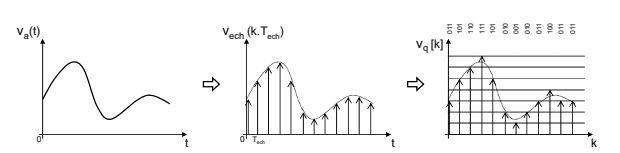
\includegraphics[scale=1]{Ech-Quant-Cod.jpg}
\captionof{figure}{Echantillonnage-Quantification-Codage \cite{CoursConv}}
\end{center}
On distingue deux grandes familles de CAN basées sur deux approches différentes du processus d'échantillonnage : les \emph{CAN classiques} dont la fréquence d'échantillonnage est telle que le
spectre du signal converti occupe quasiment toute la bande de Nyquist (Nyquist Rate ADC) et
les CAN à sur-échantillonnage (Oversampling ADC) dont seule une partie réduite du bruit de
quantification (erreur de quantification) affecte le signal converti \cite{CoursConv}.\\
Si la fréquence d'échantillonnage est bien choisie, la seule erreur introduite au cours du processus de
numérisation résulte de l'approximation faite en codant un nombre infini de valeurs analogiques par un
nombre fini $ 2^{n} $ de niveaux binaires. Le numérique n'est donc évidemment pas parfait, seulement on peut, en augmentant le nombre de bits $ n $, diminuer autant qu'on veut l'erreur introduite par la
numérisation. Avec , comme objectif, de maintenir l'erreur de quantification en dessous du seuil
de sensibilité de l'oreille humaine. Plus le nombre de bits augmente, plus le rapport signal sur bruit \emph{SNR} s'améliore \cite{Ponge}.\\
Après cette transformation, les données se dirigent vers un processeur de traitement numérique. Un traitement fait en virgule fixe est de toute évidence la plus indiquée pour être plus optimal. Il doit être considéré en cas d'implantation des algorithmes sur DSP vu que les ressources sont limitées.
\paragraph{}
Le convertisseur numérique-analogique permet de communiquer d'un système numérique vers un système
analogique. Il convertit donc un nombre binaire en une tension (ou un courant) qui lui est proportionnel.\\ L'entrée est numérique et se note formellement $ N = (b_{n-1}…b_{1}b_{0})_{2} $ avec les $ b_{i} \in \lbrace 0,1\rbrace $, $ N $ l'entrée numérique et $ n $ la résolution numérique (nombre de bits). La sortie est analogique et dans un premier temps, la conversion analogique-numérique se fait simplement par $ u_{S} = Nq + u_{S_{min}} $ avec $ u_{S} $ la tension à la sortie du convertisseur et $ q $ le \emph{ quantum ou résolution analogique} (en Volts) \cite{20Electro}.\\
Par ce qui précède on aura de toute évidence une sortie discrète du fait que les conversions sont réalisées à chaque arrivée d'un échantillon. Pour pallier à cela, le CNA a un système permettant le maintient de la tension $ u_{S} $ en sa sortie, jusqu'à l'arrivée d'un nouvel échantillon. On obtient alors en sortie, un \emph{signal analogique en escalier}. Il a ainsi un spectre fréquentiel comportant des fréquences supérieures à la fréquence maximale du signal de base. Cela est dû aux changements brusques observées pour une forme en escaliers. Il est par conséquent important de \emph{lisser} ce signal en supprimant les composantes de fréquence élevée pour obtenir finalement un signal à variations majoritairement moins brusques et/ou plus proche du signal analogique désiré.
\subsection{Filtre de lissage}
C'est le dernier élément de la chaîne de traitement du signal. Comme dit dans la section précédente, il permet de lisser le signal en escalier qu'on obtient à la sortie du CNA. Le lissage se fait par suppression des fréquences supérieures à la fréquence maximale du signal d'entrée (moitié de la fréquence d'échantillonnage). Il s'agira donc d'un filtre passe-bas comme pour le premier élément de la chaîne (filtre anti-repliement). On en illustre l'importance grâce aux figures qui suivent \cite{CoursConv} :
\begin{center}
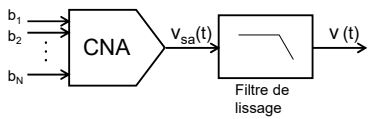
\includegraphics[scale=1]{FiltreLissage.jpg}
\captionof{figure}{Positionnement du filtre de lissage}
\end{center}
\begin{center}
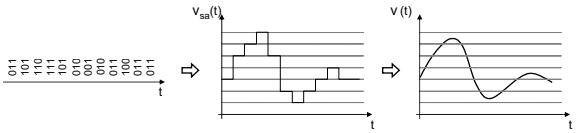
\includegraphics[scale=1]{Lissage.jpg}
\captionof{figure}{Processus complet de conversion N/A (signaux associés)}
\end{center}\newpage
\subsection{Traitement}
\paragraph{}
Une fois les données numérisées, elles sont finalement traitées. Le traitement se passe dans un processeur de traitement numérique. Il existe une multitude de processeurs, et également un grand nombre d'architectures utilisées. Néanmoins, certains processeurs sont optimisés pour le traitement du signal. Il s'agit des \emph{\textbf{DSP}} (\emph{Digital Signal Procesing}) dont on a sommairement parlé dans les parties précédentes.
\paragraph{}
Le \emph{DSP} est un microprocesseur optimisé pour exécuter des applications de traitement numérique du signal (filtrage, extraction des signaux, etc.) le plus rapidement possible. Ils sont utilisés dans la plupart des applications du traitement numérique du signal en temps réel. On les retrouve ainsi dans les modems, les téléphones mobiles, les appareils multimédia, les récepteurs GPS, les chaînes de traitement de son,... En bref, partout où l'on reçoit un signal complexe que l'on doit modifier à l'aide du filtrage. Un \emph{DSP} fournit des instructions usuelles comme la multiplication, l'addition, la soustraction, etc. Mais son jeu d'instructions est élaboré de manière à exécuter des opérations très courantes dans des algorithmes de traitement du signal les plus usuels \cite{ImageChaineTrait}.\\
Des nombreux algorithmes de traitement du signal ont par exemple besoin d'effectuer rapidement des multiplications suivies d'une addition. Les \emph{DSP} accélèrent ces genres de calcul en fournissant des instructions capables de multiplier deux nombres et d'en additionner un troisième en une seule fois (en un cycle d'horloge). Certains \emph{DSP} arrivent même à réaliser plusieurs opérations complexes de ce genre en un seul cycle d'horloge.\\
La majorité des \emph{DSP} calculent exclusivement avec des nombres à virgule fixe. L'absence d'unité en nombre flottant rend le composant meilleur marché tout en permettant une grande vitesse de traitement des données. Certains \emph{DSP} possèdent cependant des unités de calcul en virgule flottante pour des applications exigeant une large dynamique des valeurs ou une grande précision relative des résultats. Ils peuvent être combinés avec d'autres composants dans le même boîtier. C'est ainsi par exemple qu'on a, dans un même, le \emph{DSP} et les convertisseurs (\emph{Convertisseur Analogique-Numérique} et \emph{Numérique-Analogique}). \emph{Dans un appareil équipé d'un DSP, la vitesse d'exécution des calculs dans ce dernier est généralement la partie déterminante de la vitesse d'exécution du travail effectué par la machine \cite{WikiDSP}.}\newpage
\paragraph{}
Au vu de ce que nous venons de montrer dans le paragraphe précédent, le \emph{DSP} est la solution indiquée pour un système embarqué complet. Pour notre cas, sachant que nos ordinateurs sont équipés des processeurs assez rapides qui arrivent à réaliser le traitement des données avec une vitesse suffisante pour que nous testions de fonctionnement réel de notre système, nous réaliserons \emph{dans un premier temps} notre système en nous servant de l'ordinateur. Les caractéristiques utiles de ce dernier sont précisées dans la section traitant de l'élaboration de l'algorithme.\\
Il s'avère alors indubitable que, comme le traitement que nous mettons au point est un filtrage, avec comme objectif l'annulation d'écho sonore, cette partie (le traitement) suffit pour tirer des conclusions pertinentes sur le système et pour envisager (projet à long terme selon la demande ou le besoin) finalement une production du matériel conçu selon ce travail. Donc, le filtre anti-repliement et autres éléments de la chaîne de traitement du signal ne seront pas conçus par nous mais nous nous servirons de ceux de la carte son  de l'ordinateur (pour le test du fonctionnement) et ceux qui seraient couplés au boîtier du DSP (en cas de production matérielle).\\
\section{Élaboration de l'algorithme et présentation du système}
Nous allons réaliser l'annulation d'écho par utilisation de l'algorithme \emph{BPNLMS++}; les coefficients seront donc réinitialisés selon le principe illustré par les formules \ref{BPNLMS++2} et \ref{BPNLMS++1}\\
Avec $ S_{k} $ et $ S_{-k} $ définis respectivement par \\$ S_{k} = $\(\begin{pmatrix}
s(kN-p+1) & s(kN-p+2) & \cdots & s(kN+N-1)
\end{pmatrix}\)$ ^{T} $  et\\ $ S_{-k} = $\(\begin{pmatrix}
s(kN+N-1) & s(kN+N-2) & \cdots & s(kN-p+1)
\end{pmatrix}\)$ ^{T} $.\\
Les deux sont tous de longueur $ N+p-1 $ prenant directement en compte la longueur $ p $ du filtre ainsi que la taille $ N $ des blocs d'échantillons.\\
Ce qui précède nous fait immédiatement remarquer que les deux vecteurs ont les mêmes termes mais arrangés en ordre inverse. Mathématiquement, ça correspond à dire que $ S_{-k} $ s'obtient en \emph{multipliant $ S_{k} $ par une matrice carrée de dimensions adéquates et dont tous les termes sont nuls sauf la diagonale secondaire qui sera totalement constituée des $ 1 $.}\newpage
\subsection{Élaboration de l'algorithme d'apprentissage}\label{Etapes}
Soit à utiliser un processeur à $ 16 $ \emph{bits}, ce qui correspond au dernier nombre premier de Fermat, le cinquième pour être exact. En effet, si nous choisissons $ b=16 $, ça veut dire que dans la forme canonique des nombres de Fermat introduits à la sous-section \ref{NbrFermat} nous avons que $ t=4 $, soit donc que le nombre de Fermat en question est $ 2^{2^{4}}+1 = 2^{16}+1 = 65537 = F_{4}$ . Ce choix est judicieux vu que nous comptons faciliter les calculs par transformée en nombres de Fermat (FNT), car là on a bel et bien un nombre de Fermat valable (un nombre premier en l'occurrence et en plus le plus grand nombre premier de Fermat connu).\\
Aussi, étant donné ce que nous avons considéré à la sous-section \ref{MetALPHA}, entre autres les définitions selon lesquelles $ M = 2^{t+1-i} $ et $ \langle\alpha = 2^{2^{i}}\rangle_{F_{t}} $, en choisissant par exemple $ i=-2 $ on obtient une longueur de transformation $ M=128 $ et $ \langle\alpha = \sqrt[4]{2}\rangle_{F_{4}} = 4938 $.\\
Voulant conserver le fait selon lequel on ne peut pas transformer une séquence de longueur supérieure à la longueur $ M $ de la transformée, nous devons faire remarquer que vu que $ S_{k} $ et $ S_{-k} $ sont de longueur $ N+p-1 $, on doit impérativement respecter la condition $ M\geq N+p-1 $ ou alors prendre $ N+p-1 < M $ pour le compléter ensuite jusqu'à la longueur $ M $. Alors, pour choix on peut prendre par exemple $ N=64 $ et $ p=64 $ (deux moitiés de $ M $). Sur base de cela, nous aurons les étapes de l'algorithme :
\begin{itemize}
\item[1°)] \textbf{Acquisition et préparation du signal à manipuler;}\\
\item[2°)] \textbf{Écriture des fonctions qui réalisent la FNT et son inverse}\\
Après extraction du signal, nous pourrons être amenés à effectuer une transformée en nombres de Fermat sur le vecteur constitué des échantillons. Pour cela, nous devons réaliser ce qui suit:
\begin{itemize}
\item[1.] Fonction réalisant la transformée de la séquence de longueur fixée $ M $;
\item[2.] Fonction réalisant la transformée inverse d'une séquence de longueur identique;
\end{itemize}\newpage
\item[3°)] \textbf{Écriture d'une boucle devant réaliser l'apprentissage (adaptation du filtre) :}
\begin{itemize}
\item[1.] Fenêtrage d'un bloc de $ 64 $ échantillons du signal d'entrée;
\item[2.] Construction globale du signal d'entrée à considérer $ S_{k} $ en faisant précéder les $ 64 $ échantillons de $ p-1 $ derniers échantillons provenant du signal $ S_{k-1} $;
\item[3.] Vu qu'ainsi on a $ S_{k} $ de longueur $ M=128 $ termes en le complétant, calcul de sa FNT par appel de la procédure correspondante;
\item[4.] Initialisation des coefficients du filtre (comme notre filtre est de longueur $ p=64 $, nous prendrons pour filtre initial, un filtre dont tous les $ 64 $ termes sont tous nuls);
\item[5.] Complément des coefficients du filtre par des 0 par ajout de $ M-p $ termes nuls pour obtenir un vecteur pouvant subir une FNT de longueur $ M $;
\item[6.] Calcul de la FNT du vecteur ainsi formé par appel de la procédure correspondante;
\item[7.] Calcul du produit terme à terme de ces deux FNT précédemment obtenus (Transformée de $ W_{k} $ complété multipliée par la transformée de $ S_{k} $;
\item[8.] Calcul de la FNT inverse du produit obtenu par appel de la procédure dédiée (cela donne le produit de convolution des coefficients du filtre par le signal d'entrée. Donc on obtient $ y_{w_{k}} $ dont seuls les $ N $ derniers termes correspondent aux $ N $ vrais échantillons formant $ y_{w_{k}} $;
\item[9.] Formatage de $ y_{w_{k}} $ par élimination des $ M-N $ premiers termes inutiles. Pour cela, on multiplie une matrice de taille $ N\times M $ dont les $ M-N $ premiers termes de chaque ligne sont tous nuls et l'autre partie est semblable à une matrice unitaire de taille $ N $ (c'est-à-dire que tous ses termes diagonaux sont égaux à $ 1 $) par le vecteur $ y_{w_{k}} $ obtenu après la transformation inverse de l'étape précédente ; on obtient après cette multiplication, une matrice $ N\times 1 $ qui correspond effectivement au vrai vecteur $ y_{w_{k}} $ recherché;
\item[10.] Calcul du vecteur d'erreur par comparaison (une différence) de la valeur trouvée $ y_{w_{k}} $ avec la valeur désirée $ y_{k} $;
\item[11.] Complément de ce vecteur par des 0 jusqu'à obtenir un vecteur de longueur $ M $ car c'est bien cela la longueur de la transformée que nous avons choisi d'utiliser (on aura ajouté alors $ M-N $ termes nuls);
\item[12.] Calcul de la FNT du vecteur d'erreur ainsi complété;
\item[13.] Construction du vecteur image $ S_{-k} $ en multipliant le vecteur $ S_{k} $ déjà bien formaté et complété par une matrice de taille $ M $ (matrice carrée donc) dont tous les termes sont nuls à part ceux de la diagonale secondaire qui sont tous égaux à $ 1 $. La multiplication de cette dernière matrice par $ S_{k} $ a donc pour effet de renverser l'ordre de ses termes;
\item[14.] Calcul de la FNT de ce vecteur image;
\item[15.] Calcul du produit terme à terme de ce vecteur image transformé avec le vecteur d'erreur transformé;
\item[16.] Calcul de la transformée inverse du résultat ainsi obtenu (la réponse correspond au vecteur $ \varepsilon_{k}\ast S_{-k} $ dont seuls les $ p $ derniers termes forment le vrai vecteur recherché;
\item[17.] Formatage du résultat obtenu en lui appliquant une matrice que nous nommons $ E $, de dimension $ p\times M $ pour obtenir au final un vecteur de taille $ p $. Pour cela on multiplie la matrice construite $ E $ par le résultat obtenu à l'étape précédente. Cette matrice en est en fait une dont les $ M-p $ premiers termes de chaque ligne sont nuls et l'autre partie est comme une matrice carré de taille $ p\times p $ dont les termes de la diagonale principale sont tous égaux à $ 1 $ et les autres sont tous nuls (matrice unitaire de taille $ p $);
\item[18.] Calcul du produit terme à terme du vecteur d'entrée $ S_{k} $ transformé  avec son vecteur image $ S_{-k} $ aussi transformé;
\item[19.] Calcul de la transformée inverse du précédent produit (cela nous permet d'obtenir la fonction d'autocorrélation du signal d'entrée $ R_{ss}(k) = S_{k}\ast S_{-k} $ qui est aussi réduit à ses $ p $ derniers termes en lui appliquant la matrice $ E $ comme cela a été fait à l'étape $ 17 $;
\item[20.] Construction de la matrice diagonale $ G_{k} $ de taille $ p\times p $ tel qu'elle fut définie à la sous-section \ref{MatrGk};
\item[21.] Calcul des vecteurs $ G_{k}.(\varepsilon_{k}\ast S_{-k}) $ et $ G_{k}.R_{ss}(k) $;
\item[22.] Réinitialisation des coefficients du filtre en appliquant l'algorithme \emph{BNLMS} (tout en tenant compte de la dernière remarque de sur l'état formel des formules du \emph{BNLMS} et du \emph{BPNLMS}). On appliquera donc précisément \\
 \\
\begin{center}
$ W_{k+1}(i)=W_{k}(i)+\frac{\lambda}{[R_{ss}(k)](i)+\beta}[(\varepsilon_{k}\ast S_{-k})](i) $
\end{center};
\item[23.] Réinitialisation des coefficients du filtre en appliquant l'algorithme \emph{BPNLMS} en tenant également compte du fait que la formule s'exprime réellement par :\\
 \\
\begin{center}
$ W_{k+1}(i)=W_{k}(i)+\frac{\lambda}{[G_{k}R_{ss}(k)](i)+\beta}[G_{k}(\varepsilon_{k}\ast S_{-k})](i) $
\end{center};
\item[24.] Construction du vrai vecteur des coefficients du filtre en prenant tous les termes impairs égaux aux termes impaires correspondants du vecteur trouvé à l'étape précédente et les termes pairs aux termes pairs correspondant du vecteur trouvé à l'étape $ 22 $ (ainsi on vient de réinitialiser le filtre en appliquant le \emph{BPNLMS++});
\item[25.] Relance de la boucle jusqu'au nombre d'itérations voulu.
\end{itemize}
\item[4°)] \textbf{Fin de la boucle, renvoi des valeurs figées des coefficients du filtre en les formatant si nécessaire}\\
\end{itemize}
\subsection{Présentation du système réel}
Après cette étape d'apprentissage, on obtiendra les coefficients du filtre qui modélisent au mieux la réponse impulsionnelle de l'enceinte considérée. Ainsi, comme mentionné à la sous-section \ref{Convol}, le signal d'écho obtenu dans l'enceinte considérée peut bel et bien aussi s'obtenir,dans les mêmes conditions, par convolution du signal d'entrée avec le vecteur formé des coefficients du filtre ainsi construit. Cette solution est cruciale et déterminante pour l'efficacité et la rapidité\footnote{Sans ignorer les autres avantage d'un système d'annulation d'écho tout court.} des systèmes de communication. En effet, annuler directement l'écho grâce à un modèle numérique équivalent à l'enceinte utilisée, nous permet :
\begin{itemize}
\item[•] De ne pas avoir à empêcher un locuteur de parler lorsque l'autre parle;
\item[•] De simuler l'écho venant de n'importe quelle source (sélectionner un signal en particulier dont on veut extraire l'écho) pour ensuite le soustraire du signal qu'on compte transmettre.
\end{itemize}
Ce qui serait carrément impossible sans cette modélisation de la réponse de la salle.
\paragraph{}
Le système se résume donc ainsi :\\
Deux interlocuteurs ayant chacun un combiné de communication, équipés chacun d'un système d'annulation d'écho, sont dans deux enceintes différentes (et dans la même enceinte à la limite ; mais c'est sans intérêt). On procède premièrement à une phase d'apprentissage où, un son de quelques secondes est émis par le haut-parleur des combinés de chaque locuteur et le filtre de chaque combiné est mis à jour. Ensuite s'établit la communication entre les deux interlocuteurs où, chaque fois que l'une des sources émet un signal, on en soustrait la modélisation de l'écho du signal venant de l'autre. Ainsi, aucun des deux ne peut réentendre sa voix à travers son haut-parleur. Cela résout le problème d'écho acoustique associé au système de communication considéré.\\ Dans la suite (pour les essais) nous n'allons considérer qu'un interlocuteur.Pour cela, le signal venant de l'autre sera juste appelé \emph{signal lointain} et celui qui vient du locuteur présent dans la salle d'expérimentation sera dit \emph{signal local}. Cela nous permettra de réaliser l'adaptation du filtre et de vérifier si le filtre obtenu modélise bel et bien l'enceinte prototype.
\section{Implémentation de l'algorithme et simulations}
Dans cette section, nous allons écrire l'algorithme élaboré dans la section précédente en langage Matlab (qui a évidemment une syntaxe proche du \textbf{C} et qui nous permettra aumoins de réaliser des expérimentations de manière moins complexe).\\
Utilisant un processeur à virgule flottante (celui de l'ordinateur), nous n'allons pas nous cramponner sur le formatage du signal d'entrée. Par conséquent, la transformation de Fourier va suffire pour avoir un aperçu de l'algorithme global.
\subsection{Traitement brut des données}\label{Brut}
Ce traitement revient à réaliser l'adaptation des coefficients du filtre à la manière dont la théorie a été élaborée au début du second chapitre. Donc sans optimiser le temps de calcul avec un traitement par blocs. Nous allons donc réaliser un algorithme d'adaptation évoluant échantillon par échantillon et non par blocs. Ceci est utile pour remarquer la précision de ce traitement malgré le manque de robustesse et la charge de calcul. L'algorithme élaboré pour cet effet est ,sous \textbf{Matlab}, donné par l'annexe \ref{Anne1} .\\
La compilation de ce code a duré $ 12.424632 $ \emph{secondes} (valeur donnée par le chronomètre intégré à Matlab en excluant la prise du son) pour un signal d'entrée pris enregistré sur $ 40 $ \emph{secondes} (voir la ligne $ 12 $ de ce code) pour pouvoir pousser très loin l'adaptation (jusqu'à $ 20850 $ tours de boucle principaux comme on le voit à la ligne $ 43 $ de ce code).\\
Le signal d'entrée, avec \textit{les niveaux de son représentés en fonction des numéros d'échantillon}, était le suivant :
\begin{center}
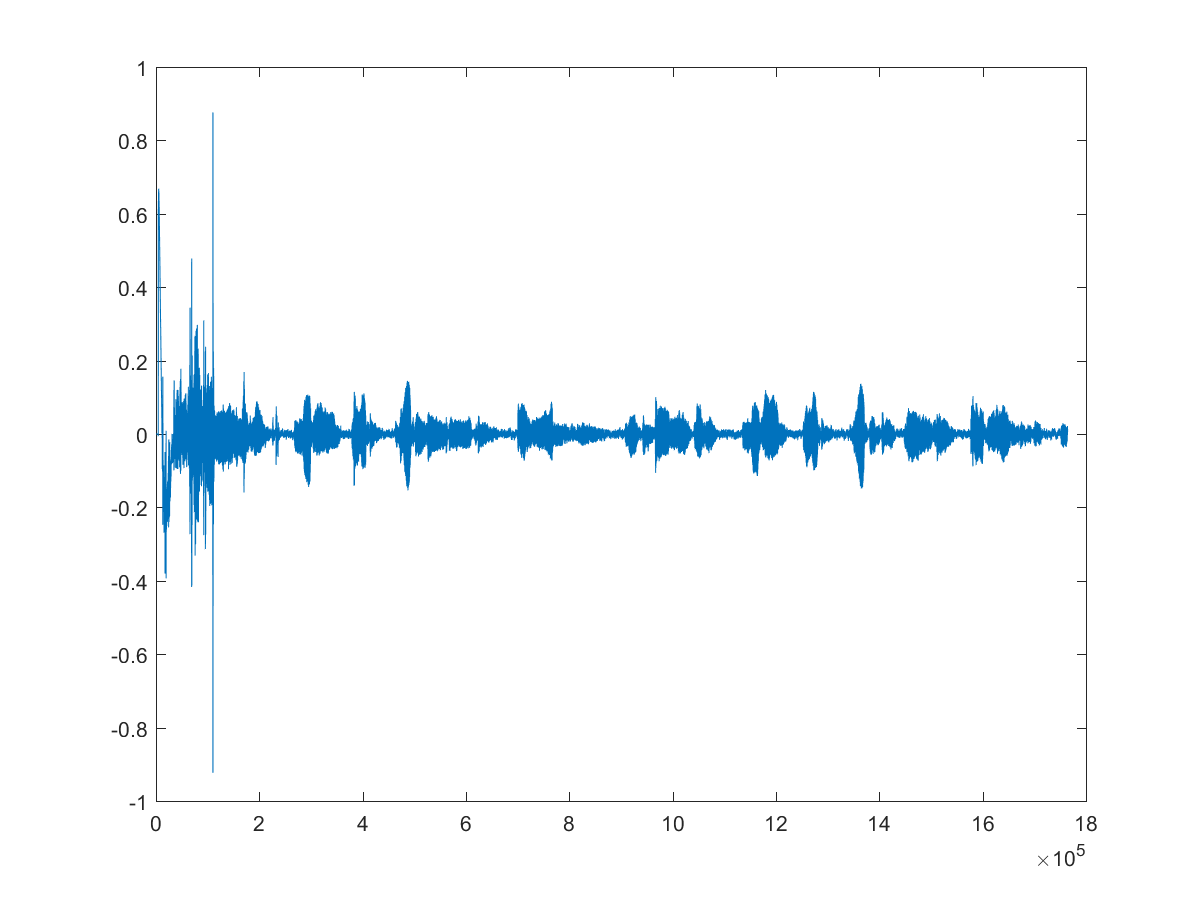
\includegraphics[scale=0.7]{Entree.png}
\captionof{figure}{Signal d'entrée utilisé}
\label{entree}
\end{center}
Le signal présenté sur la figure \ref{entree} a été obtenu en nous enregistrant pendant $ 40 $ \textit{secondes} entrain de chanter de façon arbitraire juste pour le test. Et cela a été ensuite tracé en utilisant \textit{Matlab} (voir les annexes \ref{Anne1} et \ref{Anne2}).\\
Pour $ i=20850 $ tours de boucles (voir la ligne $ 43 $ du code), nous avons obtenu \textit{les coefficients du filtre représentés en fonction des numéros d'échantillons} par: 
\begin{center}
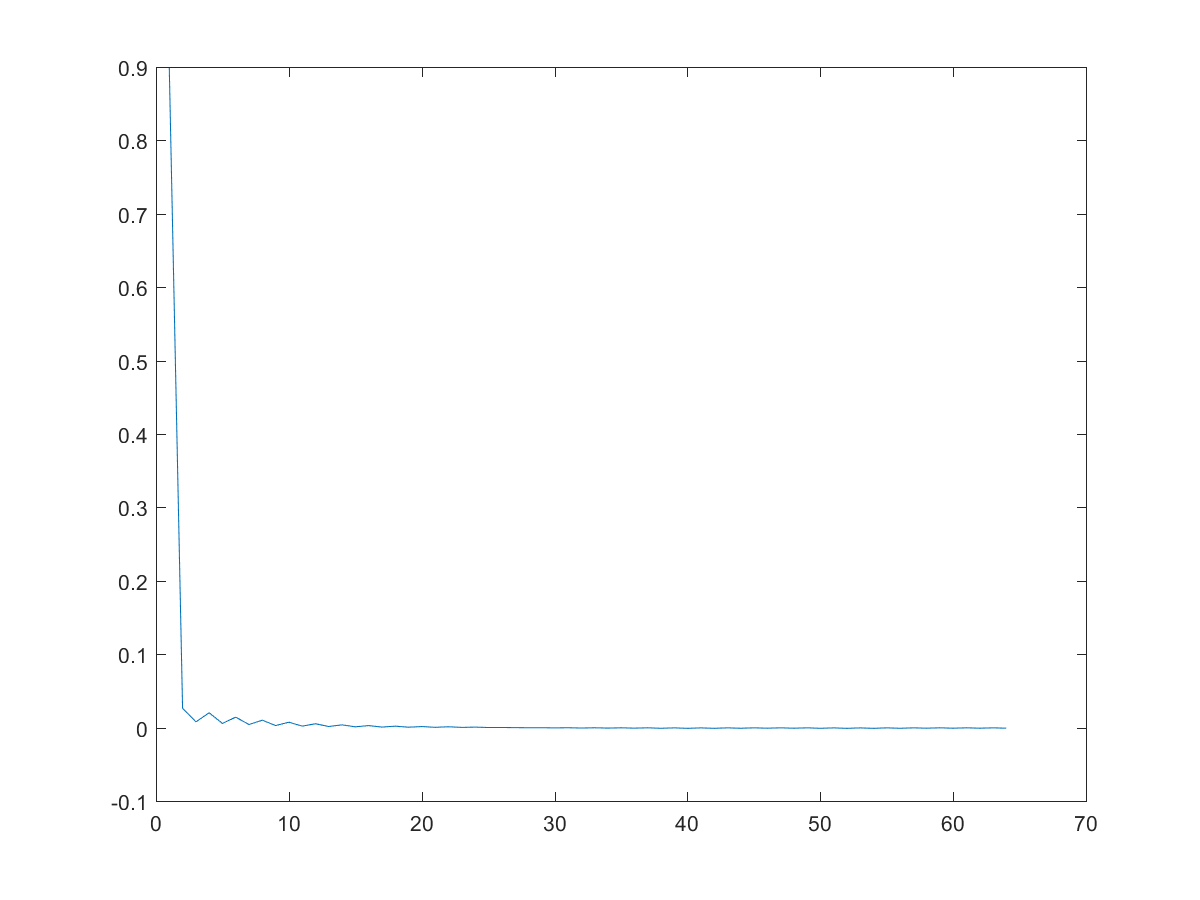
\includegraphics[scale=0.7]{Filtre1.png}
\captionof{figure}{Valeurs des $ 64 $ coefficients du filtre}
\label{f1}
\end{center}
Sous cette forme, sur la figure \ref{f1}, on a remarqué que la convergence du filtre est relativement lente bien que le résultat soit plus parfait. Cela sera plus clairement compris avec les sections qui suivent.
\subsection{Traitement par bloc des données}\label{Bloc}
L'algorithme utilisé et qui suit les étapes décrites précédemment (à la section \ref{Etapes} qui concerne l'élaboration de l'algorithme conseillé pour un implantation sur DSP) est donné à l'annexe \ref{Anne2} .\\
Il est très important de signaler que bien que les étapes décrites lors de l'élaboration textuelle de l'algorithme soient faites pour le cas d'un traitement par FNT et \emph{pour un processeur à virgule fixe fonctionnant sous $ 16 $ bits}, le fait que nous ayons utilisé un processeur sous $ 64 $ \emph{bits} et la transformée de Fourier est tout à fait admissible. L'algorithme textuel a juste été élaboré pour considérer le cas le plus général et pour nous guider dans l'implémentation, surtout que cela permet également d'optimiser à la fois les coûts et l'exploitation des ressources.\\ 
On remarque des simplifications drastiques en ce qui concerne le formatage des vecteurs. C'est ainsi qu'à la ligne $ 73 $ de ce code (annexe \ref{Anne2} ), on remarque qu'au lieu de multiplier le vecteur à $ 128 $ termes par une matrice particulière $ E $ (comme nous le suggère le point $ 3 $ en son étape $ 17 $ de la sous-section \ref{Etapes} sur les étapes de l'algorithme), \textbf{Matlab} nous permet d'extraire très simplement ces derniers termes. C'est le cas également aux lignes $ 62 $ et $ 77 $ (annexe \ref{Anne2} toujours)  où les manipulations sont grandement simplifiées par rapport à ce que nous proposions au préalable. Ces propositions ont tout de même le mérite d'être plus générales comme méthode et donc utilisables même quand le langage ne permet pas une manipulation très simple des matrices.\\
La compilation de ce code a duré $ 8.219884 $ \emph{secondes} (valeur donnée par le chronomètre intégré à Matlab en excluant la prise du son) pour le même signal d'entrée que précédemment (voir la ligne $ 12 $ de ce code et la figure \ref{entree}) pour pouvoir pousser très loin l'adaptation.\\
Ainsi on a obtenu \textit{en fonction des numéros d'échantillons le filtre} suivant:
\begin{center}
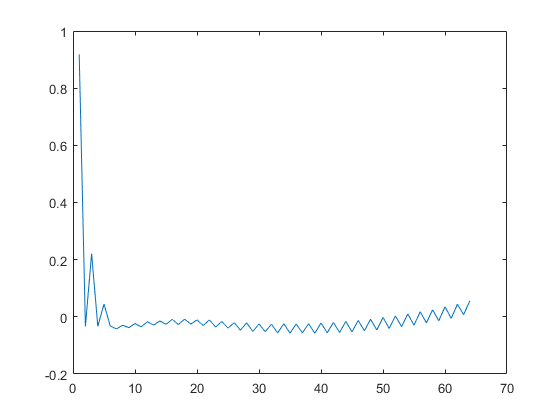
\includegraphics[scale=1]{Filtre2.png}
\captionof{figure}{Les $ 64 $ coefficients du filtre 2}
\label{f2}
\end{center}
Le filtre (ses coefficients) obtenu sur la figure \ref{f2} par contre est moins précis mais s'obtient plus vite à cause de la grande vitesse de convergence des algorithmes de traitement par bloc. Normalement, suite aux manipulations des vecteurs, on obtient un \emph{filtre renversé et décalé} comme on le voit sur cette figure:
\begin{center}
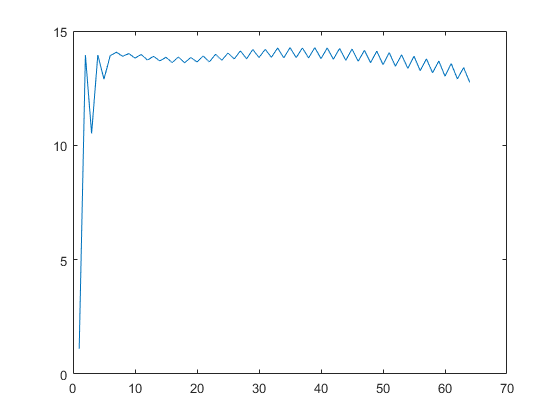
\includegraphics[scale=0.9]{Filtre2Ren.png}
\captionof{figure}{Les $ 64 $ coefficients du filtre 2 non formatés}
\label{fR}
\end{center}
De cela on obtient très aisément la courbe recherchée trouvée à la figure \ref{f2} grâce au formatage des coefficients, réalisé avec le bout de code de la ligne $ 112 $ (annexe \ref{Anne2} ) donné par:
\begin{verbatim}
w=((ones(1,64))*(mean(w))-(w))/(mean(w));
\end{verbatim}
Pour réaliser ce formatage, il suffit de détecter la valeur moyenne (on écrit \textbf{mean(w)}). Pour notre signal d'entrée, le filtre non formaté avait pour moyenne $ (13.5) $ (voir la figure \ref{fR}).
\subsection{Essais comparés}\label{essais}
Essayons, pour le même signal d'entrée (figure \ref{entree}), de trouver les coefficients du filtre pour les deux cas en considérant différentes valeurs de $ i $ (nombre d'itérations qu'on voit aux lignes $ 43 $ des codes qu'on a aux annexes \ref{Anne1} et \ref{Anne2} ) et observons l'évolution des coefficients. Nous prendrons des valeurs inférieures à $ 20850 $ car pour une boucle allant trop au delà, nous risquons de dépasser la longueur maximale des vecteurs. Notons que le signal d'entrée formaté sous forme vectorielle était de taille $ 1764352 $ échantillons.
\begin{itemize}
\item[1°)] Pour $ i=10000 $ on obtient:
\begin{center}
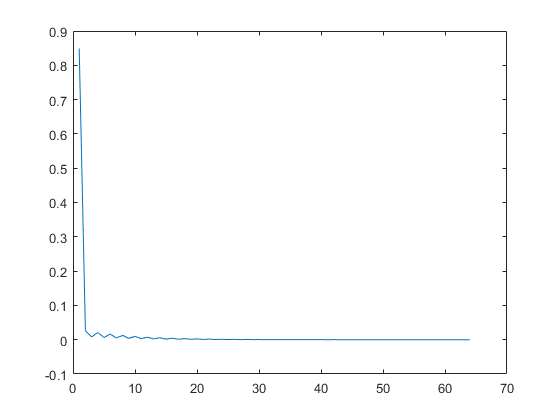
\includegraphics[scale=0.5]{Filtre1-10000.png}
\captionof{figure}{Coefficients du filtre 1 pour 10000 itérations}
\label{f1-10000}
\end{center}
Sur la figure \ref{f1-10000} on voit les coefficients du filtre, obtenus après $ i=10000 $ itérations par l'algorithme de traitement échantillon par échantillon (ce qui a duré $ 6.073958 $ secondes). On a pratiquement le bon filtre.
\begin{center}
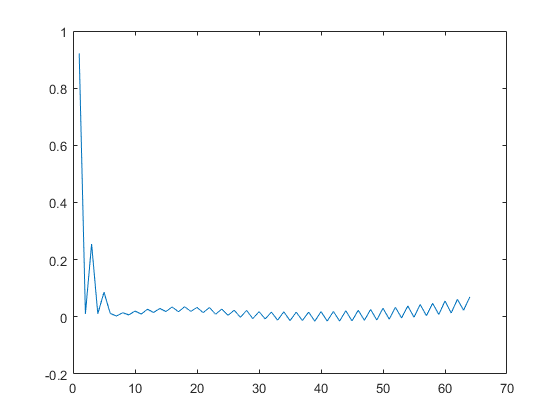
\includegraphics[scale=0.5]{Filtre2-10000.png}
\captionof{figure}{Coefficients du filtre 2 pour 10000 itérations}
\label{f2-10000}
\end{center}
Sur la figure \ref{f2-10000} on voit les coefficients du filtre, obtenus après $ i=10000 $ itérations par l'algorithme de traitement par blocs d'échantillons (ce qui a duré $ 3.920202 $ secondes, presque la moitié du temps nécessaire au traitement brut précédent).  C'est pratiquement les mêmes coefficients que ceux obtenus pour le cas où le nombre d'itérations était $ 20850 $.
\item[2°)] Pour $ i=1000 $ on obtient:
\begin{center}
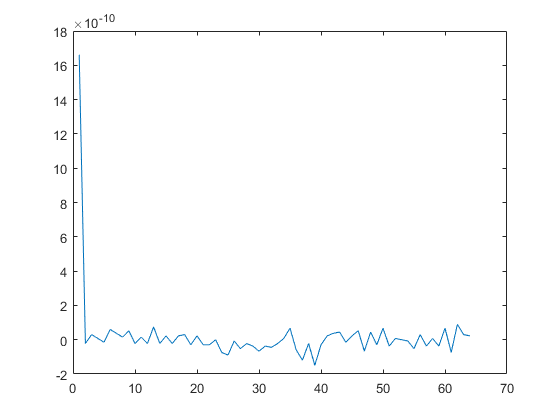
\includegraphics[scale=0.5]{Filtre1-1000.png}
\captionof{figure}{Coefficients du filtre 1 pour 1000 itérations}
\label{f1-1000}
\end{center}
Sur la figure \ref{f1-1000} on voit les coefficients du filtre, obtenus après $ i=1000 $ itérations par l'algorithme de traitement échantillon par échantillon (a duré $ 0.658588 $ secondes). Malgré que la forme est bonne, les coefficients sont très faibles.
\begin{center}
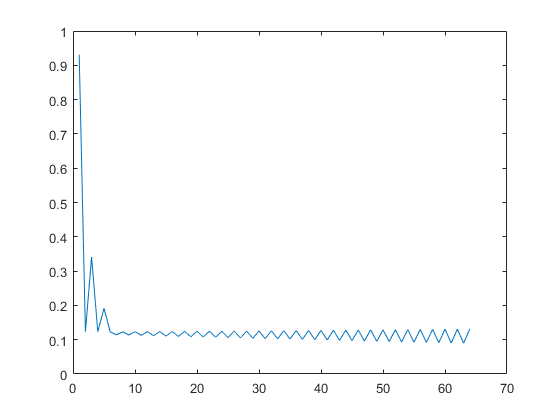
\includegraphics[scale=0.5]{Filtre2-1000.png}
\captionof{figure}{Coefficients du filtre 2 pour 1000 itérations}
\label{f2-1000}
\end{center}
Sur la figure \ref{f2-1000} on voit les coefficients du filtre, obtenus après $ i=1000 $ itérations par l'algorithme de traitement par blocs d'échantillons (pour un temps de calcul de $ 0.426955 $ secondes).  Malgré un léger décalage vers le haut, on a obtenu pratiquement le filtre final.
\item[3°)] Pour $ i=100 $ on obtient:
\begin{center}
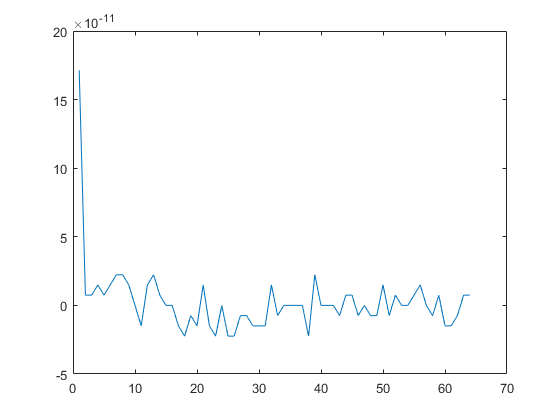
\includegraphics[scale=0.5]{Filtre1-100.png}
\captionof{figure}{Coefficients du filtre 1 pour 100 itérations}
\label{f1-100}
\end{center}
Sur la figure \ref{f1-100} on voit les coefficients, obtenus après $ i=100 $ itérations par l'algorithme de traitement échantillon par échantillon (durée de compilation de $ 0.079877 $ secondes). Malgré que la forme commence déjà à se dessiner, les coefficients sont très faibles (c'est un filtre à coefficients quasi nuls).
\begin{center}
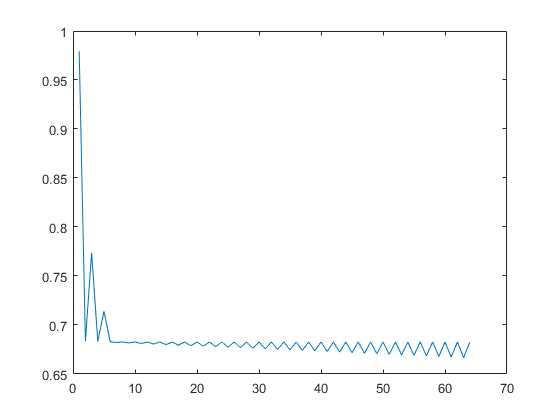
\includegraphics[scale=0.5]{Filtre2-100.png}
\captionof{figure}{Coefficients du filtre 2 pour 100 itérations}
\label{f2-100}
\end{center}
Sur la figure \ref{f2-100} on voit les coefficients du filtre, obtenus après $ i=100 $ itérations par l'algorithme de traitement par blocs d'échantillons (ce qui a duré $ 0.057885 $ secondes). La forme commence déjà à se dessiner mais les coefficients sont encore trop décalés vers le haut.
\item[4°)] Pour $ i=10 $ on obtient:
\begin{center}
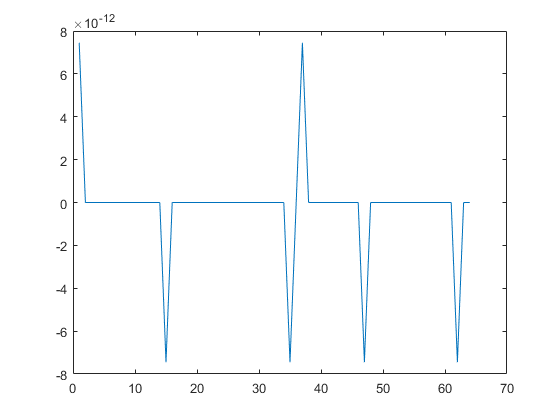
\includegraphics[scale=0.5]{Filtre1-10.png}
\captionof{figure}{Coefficients du filtre 1 pour 10 itérations}
\label{f1-10}
\end{center}
Au début de l'adaptation du filtre , les coefficients sont très mauvais. La figure \ref{f1-10} représente l'adaptation du filtre échantillon par échantillon après $ 10 $ itérations. 
\begin{center}
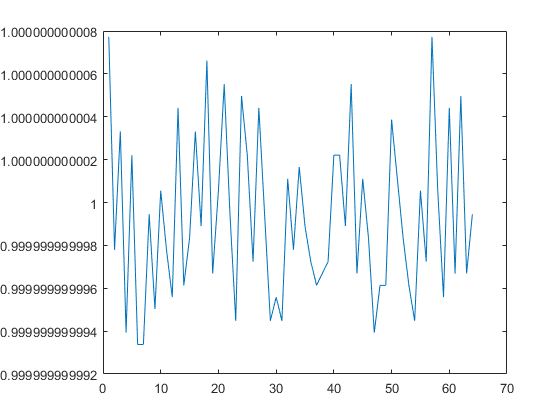
\includegraphics[scale=0.5]{Filtre2-10.png}
\captionof{figure}{Coefficients du filtre 2 pour 10 itérations}
\label{f2-10}
\end{center}
Au début de l'adaptation du filtre, les coefficients sont très mauvais. Pour $ 10 $ itérations, avec le traitement par blocs, on n'a toujours pas même l'esquisse des valeurs souhaitées, comme on peut le voir sur la figure \ref{f2-10}.
\item[4°)] Il y a également deux valeurs particulières pour les deux implémentations, les valeurs de $ i $ auxquels les filtres auront presque complètement atteint les coefficients escomptés. Après plusieurs essais on obtient:
\begin{itemize}
\item[•] $ i=4370 $ pour le filtre en traitement brut (filtre 1)
\begin{center}
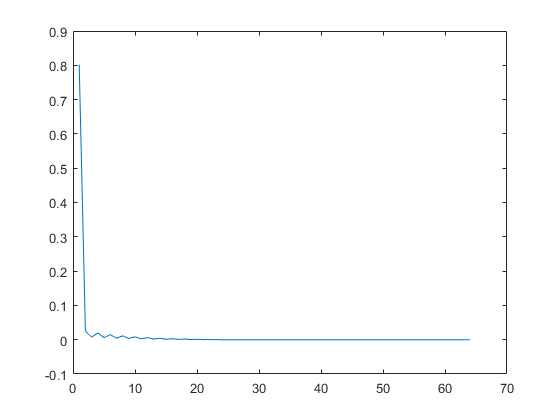
\includegraphics[scale=0.7]{Filtre1Bon.png}
\captionof{figure}{Coefficients du filtre 1 pour 4370 itérations}
\label{f1b}
\end{center}
L'algorithme de traitement échantillon par échantillon donne des très bons coefficients mais après beaucoup d'itérations ($ i=4370 $) et trop de temps ($ 3.296686 $ \emph{secondes} pour notre cas) comme on peut le voir sur la figure \ref{f1b}.
\item[•] $ i=400 $ pour celui du traitement par blocs (filtre 2)
\begin{center}
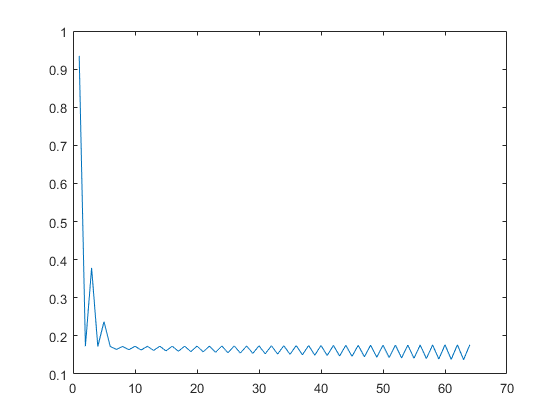
\includegraphics[scale=0.7]{Filtre2Bon.png}
\captionof{figure}{Coefficients du filtre 2 pour 400 itérations}
\label{f2b}
\end{center}
Comme on peut le voir sur la figure \ref{f1b}, l'algorithme de traitement par bloc permet d'obtenir après seulement $ 0.173829 $ \emph{secondes}, des coefficients très proches des bonnes valeurs (bien que n'étant pas très affinés, ils sont assez bons pour que le passage du signal à travers un filtre ayant des telles valeurs nous donne presqu'exactement la sortie souhaitée).
\end{itemize}
\end{itemize}
\section{Analyse des résultats et explication de l'implantation sur DSP}
\subsection{Analyse des résultats}
Ce que nous venons d'obtenir à la sous-section \ref{essais} est très crucial pour remarquer la puissance du traitement par blocs. On remarque très bien que le filtre élaboré par un traitement échantillon par échantillon n'évolue pas très vite vers les vraies valeurs, et se dégrade très vite avec la réduction du nombre d'itérations, tandis que le traitement par blocs est à la fois rapide (en terme de temps de calcul) et converge plus vite vers le filtre optimal.\\
\emph{Dans le code , à la ligne $ 61 $ pour le premier (annexe \ref{Anne1} ) et $ 64 $ (annexe \ref{Anne2} ) pour le second, on a spécifié que le résultat attendu à la sortie du filtre devait être, pour tester le fonctionnement de notre algorithme, le même signal mis à l'entrée (donc l'erreur est minimisée de manière à ce que le signal d'entrée soit le même que celui obtenu après avoir traversé le filtre). Or nous savons très bien que pour avoir une sortie identique à l'entrée, la réponse impulsionnelle du filtre doit être une impulsion toujours. Et évidemment, le filtre optimal que nous avons obtenu s'approche d'une impulsion comme on le voit très bien aux figures \ref{f1} et \ref{f2}.} \textbf{Le premier est évidemment plus proche d'une impulsion que le second bien qu'obtenu grâce à un algorithme moins robuste}. En effet, le premier algorithme, qui nous permet d'obtenir des meilleurs coefficients, converge très lentement et se dégrade très vite quand on diminue le nombre d'itérations; en plus il prend trop de temps pour donner les résultats. Pour s'en convaincre, voir les figures \ref{f1-10000} puis \ref{f1-1000} ensuite \ref{f1-100} et finalement \ref{f1-10}, on remarque très bien dans peu de temps que l'amplitude des coefficients du filtre se dégrade très vite et que les coefficients eux aussi deviennent de plus en plus écartés des bonnes valeurs jusqu'à la dégradation complète à la dernière figure, la figure \ref{f1-10}). Le second, celui obtenu grâce à l'algorithme de traitement par blocs et dont l'évolution des coefficients est représentée en ordre par les figures \ref{f2-10000} puis \ref{f2-1000} ensuite \ref{f2-100} et finalement \ref{f2-10}, est moins précis mais nettement plus robuste que le premier. En effet, il demande peu de temps de calcul et se dégrade très lentement quand on diminue le nombre d'itérations. \emph{Malheureusement, il nécessite d'importantes corrections d'erreurs.}\\
En bref, la comparaison des résultats représentés par les figures \ref{f1b} et \ref{f2b} nous montre nettement la supériorité du traitement par blocs par rapport au traitement échantillon par échantillon. On remarque très clairement la nécessité d'une implantation par blocs pour avoir un traitement en temps réel (voir les commentaires afférentes aux deux figures précédentes). 
\subsection{Explication de l'implantation sur DSP}
L'implantation sur DSP à virgule fixe et sous $ 16 $ \emph{bits} exige l'adaptation de l'algorithme élaboré (celui de l'annexe \ref{Anne2} ) de manière à ce qu'on puisse réaliser le même traitement. Pour cela, on n'a que deux choses particulières à réaliser:
\begin{itemize}
\item Formater le signal d'entrée de manière à l'adapter au processeur si nécessaire et
\item Ecrire une fonction qui réalise la transformée en nombres de Fermat tel qu'on l'a décrite et opltimisé dans les parties précédentes ainsi que son inverse. En utilisant juste les formules données.
\end{itemize}
Après avoir réalisé cela, le code sera exactement le même que celui qui a été élaboré pour le traitement par blocs en se basant sur l'esquisse qui a été faite de l'algorithme au point \ref{Etapes}. Le formatage quant à lui, quand il est nécessaire, se réalise facilement par des manipulations simples (multiplications suivies des arrondissements). Cette dernière méthode introduit évidemment une erreur mais dès qu'on envisage de l'utiliser, on peut \emph{étudier la technique adaptée pour la réduction de l'erreur qui serait introduite à la fois par ce formatage et celui réalisé durant le filtrage}. Après avoir ainsi adapté l'algorithme, il faudra alors l'écrire en \emph{assembleur} pour adapter le code à l'architecture du DSP choisi ou carrément en langage \emph{C}, laissant au compilateur le soin d'optimiser le code en l'adaptant au DSP (C'est la solution la plus simple en fait).\newpage
\section{Annulation d'écho}
Notre travail a consisté principalement à élaborer le filtre qui peut s'utiliser pour annuler l'écho dans un système de communication. Nous allons montrer la meilleure annulation que nous avons pu obtenir avec les filtres conçus. Il s'agit de l'annulation grâce au filtre implémenté par l'algorithme en annexe \ref{Anne1} qui est le plus précis (l'autre est le plus indiqué en cas d'embarquement mais nécessite d'astucieuses corrections d'erreurs). Les coefficients de ce filtre sont donnés par la figure \ref{f1}, il correspond presqu'exactement à une impulsion. On obtient d'abord la sortie et l'annulation par le code \emph{Matlab} suivant\footnote{Se référer à l'annexe \ref{Anne1} pour remarquer que \emph{myrecording} représente le signal en entrée}:
\begin{verbatim}
1-	sortie=conv(w,myrecordings);
2-	echoTransmis=(sortie(1:1608500))-(myrecordings(1:1608500));
\end{verbatim}
Ce bout de code a été exécuté à part, mais après l'exécution de celui d'adaptation pour pouvoir utiliser les mêmes variables. Il réalise en sa première ligne, la convolution du vecteur formé par les coefficients du filtre avec le signal d'entrée (c'est le filtrage si on pose que le filtre est approximativement linéaire). A la deuxième ligne on réalise alors la suppression d'écho pour le cas où le signal n'est pas trop modifié par l'enceinte (comme nous l'avons posé pour tester la validité de nos codes). On a considéré $ 1608500 $ échantillons pour ne pas risquer de dépasser la taille totale des vecteurs car le signal en entrée avait environs $ 1700000 $ échantillons.
\begin{figure}[!h]
\begin{subfigure}{.5 \textwidth}
\centering
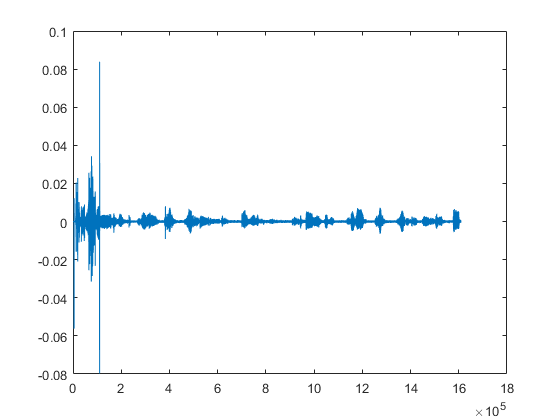
\includegraphics[scale=0.6]{Erreur.png}
\caption{Echo résiduel après filtrage.}
\label{echoAnnule}
\end{subfigure}
\begin{subfigure}{.5 \textwidth}
\centering
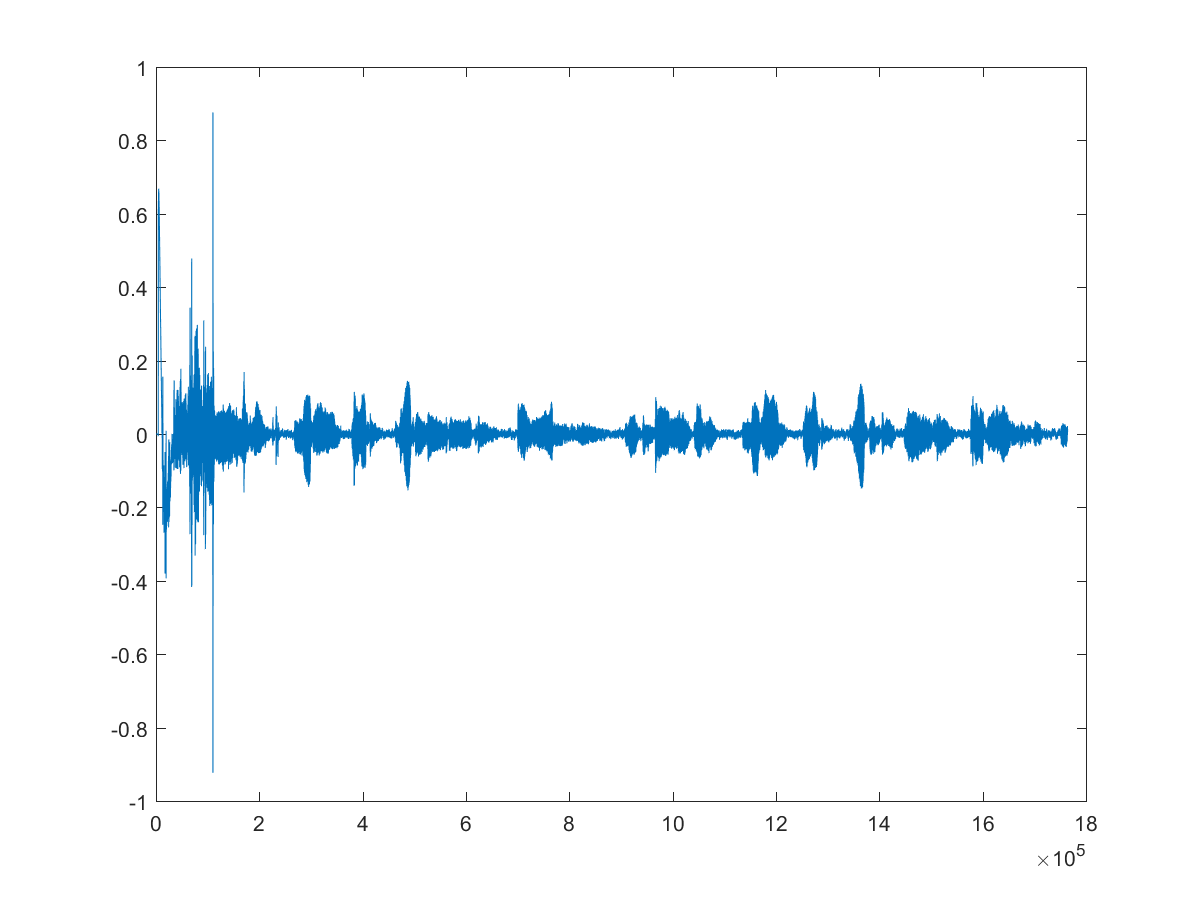
\includegraphics[scale=0.45]{Entree.png}
\caption{Echo sans filtrage.}
\label{echoNonAnnule}
\end{subfigure}
\caption{Démonstration de l'annulation d'écho}
\label{Annulation}
\end{figure}
Dans cette figure (la figure \ref{Annulation}), nous comparons l'écho reçu après filtrage du signal à envoyer à l'interlocuteur lointain, avec l'écho qu'il recevrait si le filtage n'était pas préalablement réalisé. Plus précisément, on réalise un filtrage pour modéliser l'écho, puis on le soustrait du signal à transmettre pour que l'interlocuteur lointain ne perçoive pas sa voix dans le signal qu'il recevra. Ainsi, en observant très bien les échelles des axes de ces figures, on remarque une atténuation très importante de l'écho. En effet, l'écho qui persiste après filtrage (voir la figure \ref{echoAnnule}) est environ le \emph{\textbf{dixième}} de celui qui est perçu lorsqu'aucun filtrage n'est réalisé \ref{echoNonAnnule}. Et on y voit très bien que pour ce dernier cas (absence de filtrage) l'interlocuteur lointain va entendre exactement son signal lui revenir. D'où la nécessité du filtrage.
\section{Conclusion partielle}
Dans cette dernière partie, nous avons tout d'abord décrit les éléments principaux nécessaires à l'élaboration d'un système annulateur d'écho sans prendre en compte le fait qu'il peut être incorporé à un système déjà mis en place. C'est ainsi que nous avons vu en passant la chaîne de traitement du signal et finalement nous nous sommes focalisé sur la partie concernant le traitement proprement-dit par filtrage. Cela nous a conduit à élaborer l'algorithme d'adaptation des coefficients du filtre de manière détaillée sous \textbf{Matlab} en vu d'en évaluer le fonctionnement et l'adéquation aux résultats attendus. Et bien évidemment, nous nous attendions à un filtre semblable à une impulsion  et nous l'avions obtenu de très près comme le prévoit la théorie. Nous avons finalement terminé par une illustration de l'annulation d'écho et une explication de l'implantation de l'algorithme sur DSP en système indépendant.